
%% NUIG talk 30mins
\documentclass[usenames,dvipsnames]{beamer}
\usepackage{amsmath}
\usepackage{verbatim}
\usepackage{amsfonts}
\usefonttheme[onlymath]{serif}
\usepackage{color}
\usepackage{mathtools}
\usepackage{booktabs}
%%\usefonttheme[onlymath]{serif}
%%\usepackage{tgheros}
\usepackage{tablefootnote}
\usepackage{array}
%%\usepackage{columns}
\useinnertheme{circles}
\usepackage[absolute,overlay]{textpos}

\usepackage{graphicx}


\begin{document}

\begin{frame}
\frametitle{Some models}
\texttt{poisson\textunderscore rw1\textunderscore rw1} (distribution, level process, rate process)
 \begin{align*}
 y_t &\sim \textnormal{Poisson}(\lambda_t) \\
 \ln(\lambda_{t+1}) &= \ln(\lambda_t) + \delta_t + \epsilon_t, \quad \epsilon_t \sim \textnormal{N}(0, \sigma_{\epsilon}^2) \\
  \delta_{t+1} &= \delta_t + \eta_t, \quad \eta_t \sim \textnormal{N}(0, \sigma_{\eta}^2)
\end{align*}
\small
\begin{columns}
\begin{column}{0.5\textwidth}
\textcolor{blue}{\texttt{negbin\textunderscore *\textunderscore *}}
 \begin{align*}
 y_t &\sim \textnormal{Negative binomial}(p_t,r) \\
 p_t &= \frac{r}{r+\lambda_t}
 \end{align*}
\textcolor{blue}{\texttt{*\textunderscore const\textunderscore *}}
 \begin{align*}
\ln(\lambda_{t+1}) &= \ln(\lambda_t) + \delta_t \\
\ln(\lambda_{0}) &\sim \textnormal{N}(0, 10^6) 
 \end{align*}
 \textcolor{blue}{\texttt{*\textunderscore rw2\textunderscore *}}
 \begin{align*}
\ln(\lambda_{t+1}) &= 2 \ln(\lambda_t) - \ln(\lambda_{t-1}) + \delta_t + \epsilon_t\\
 \end{align*}
\end{column}
\begin{column}{0.5\textwidth}
\textcolor{blue}{\texttt{*\textunderscore *\textunderscore const}}
 \begin{align*}
\delta_{t+1}) &= \delta_t \\
\delta_{0} &\sim \textnormal{N}(0, 10^6) 
 \end{align*}
 
\textcolor{blue}{\texttt{*\textunderscore *\textunderscore rw2}}
 \begin{align*}
\delta_{t+1} &= 2 \delta_t - \delta_{t-1} + \eta_t
 \end{align*}

\end{column}
\end{columns}

\end{frame}


\begin{frame}
 Ireland
\end{frame}

{
\usebackgroundtemplate{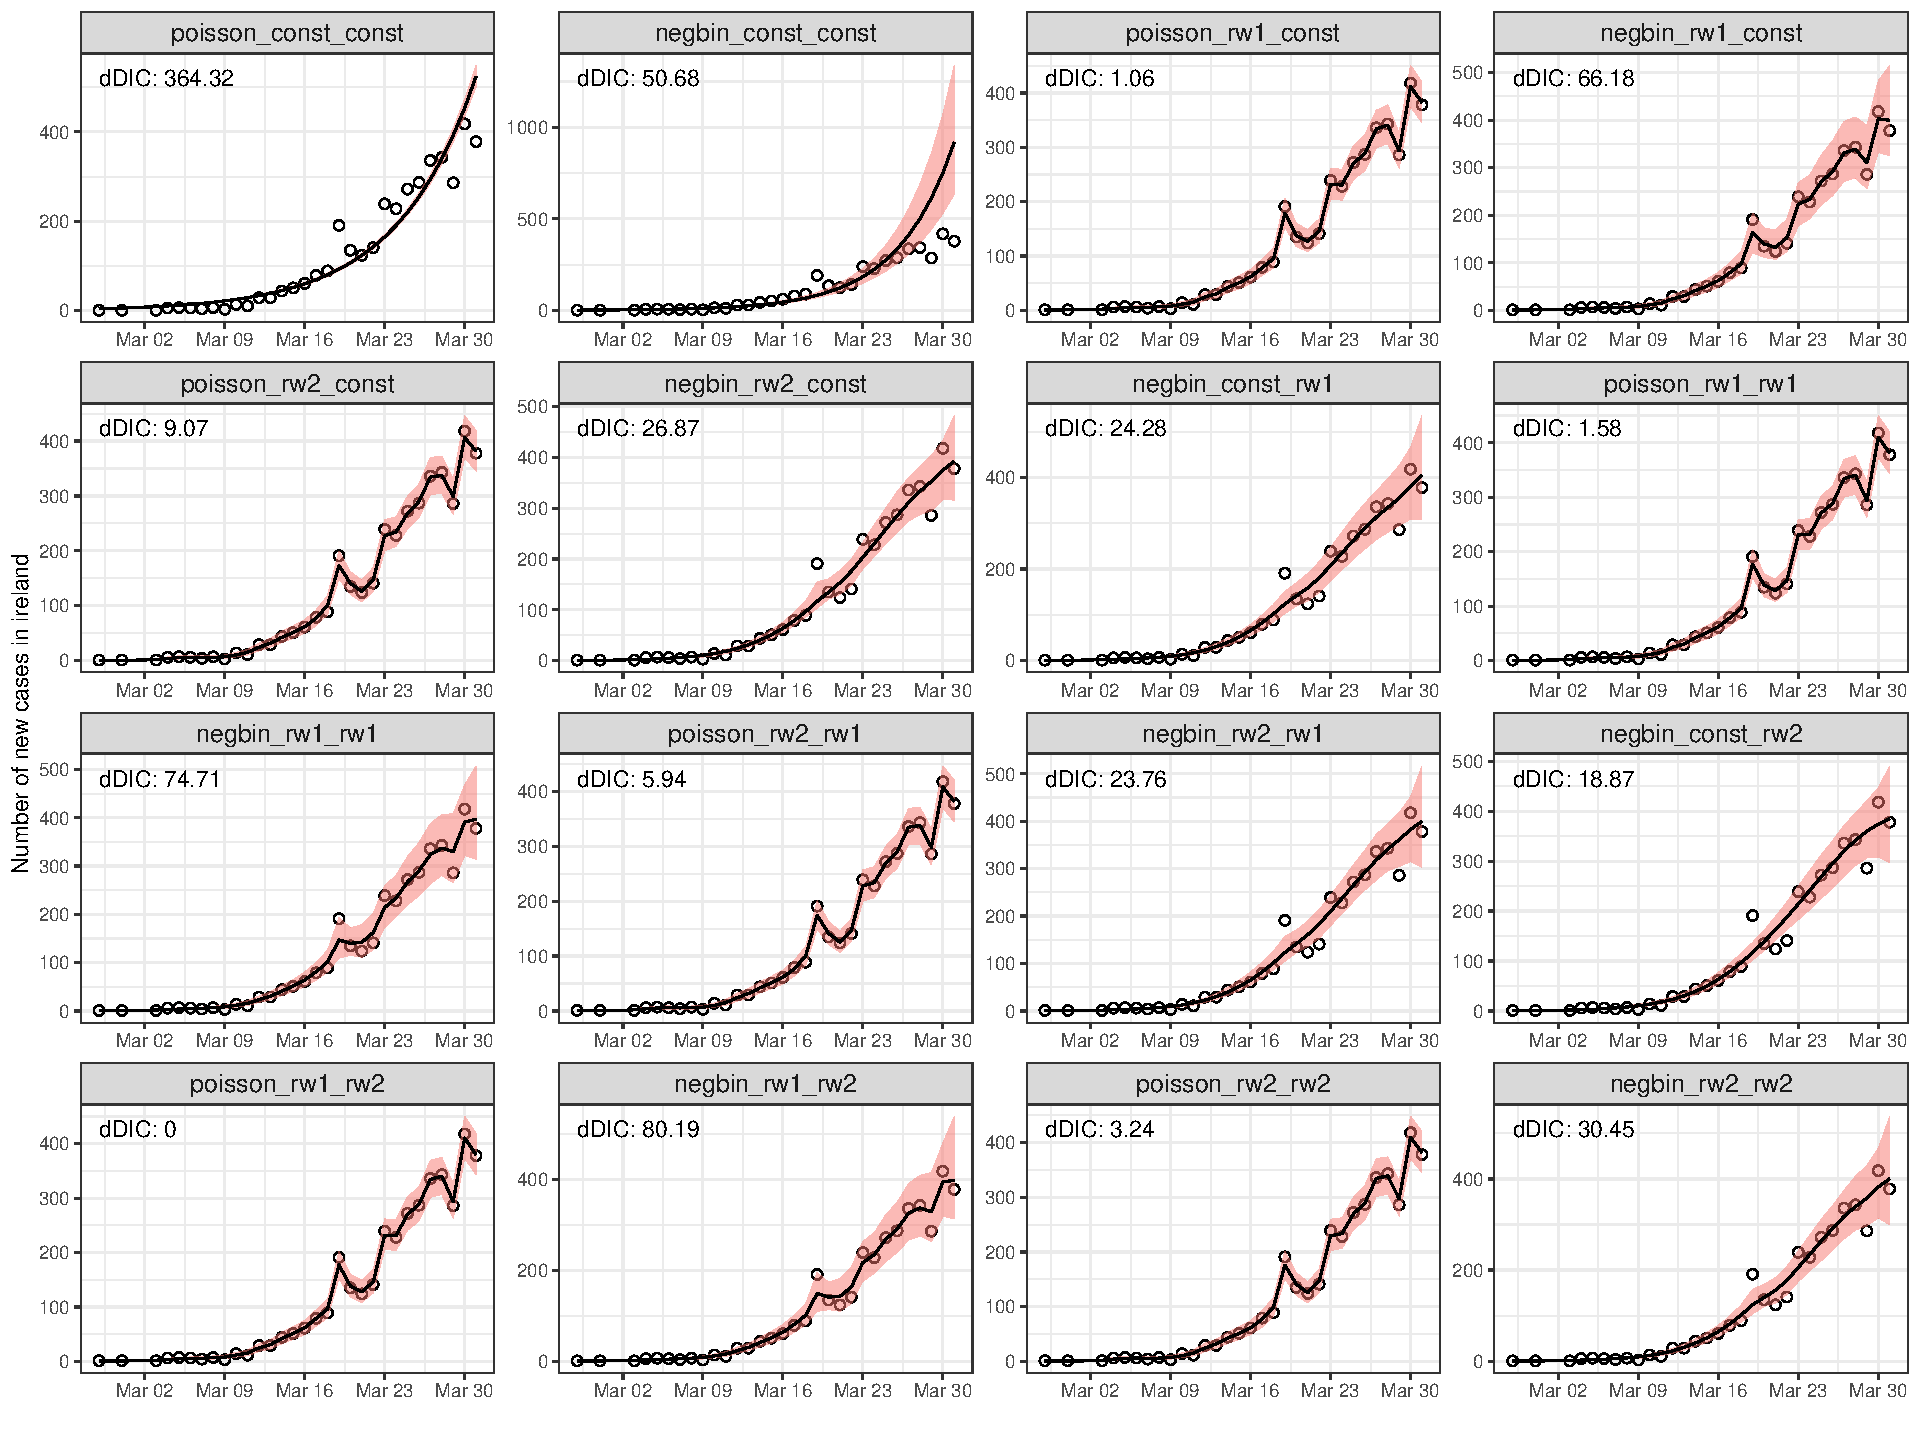
\includegraphics[width=\paperwidth]{figures/all_fits_ireland.pdf}}
\begin{frame}[plain]
\end{frame}
}

{
\usebackgroundtemplate{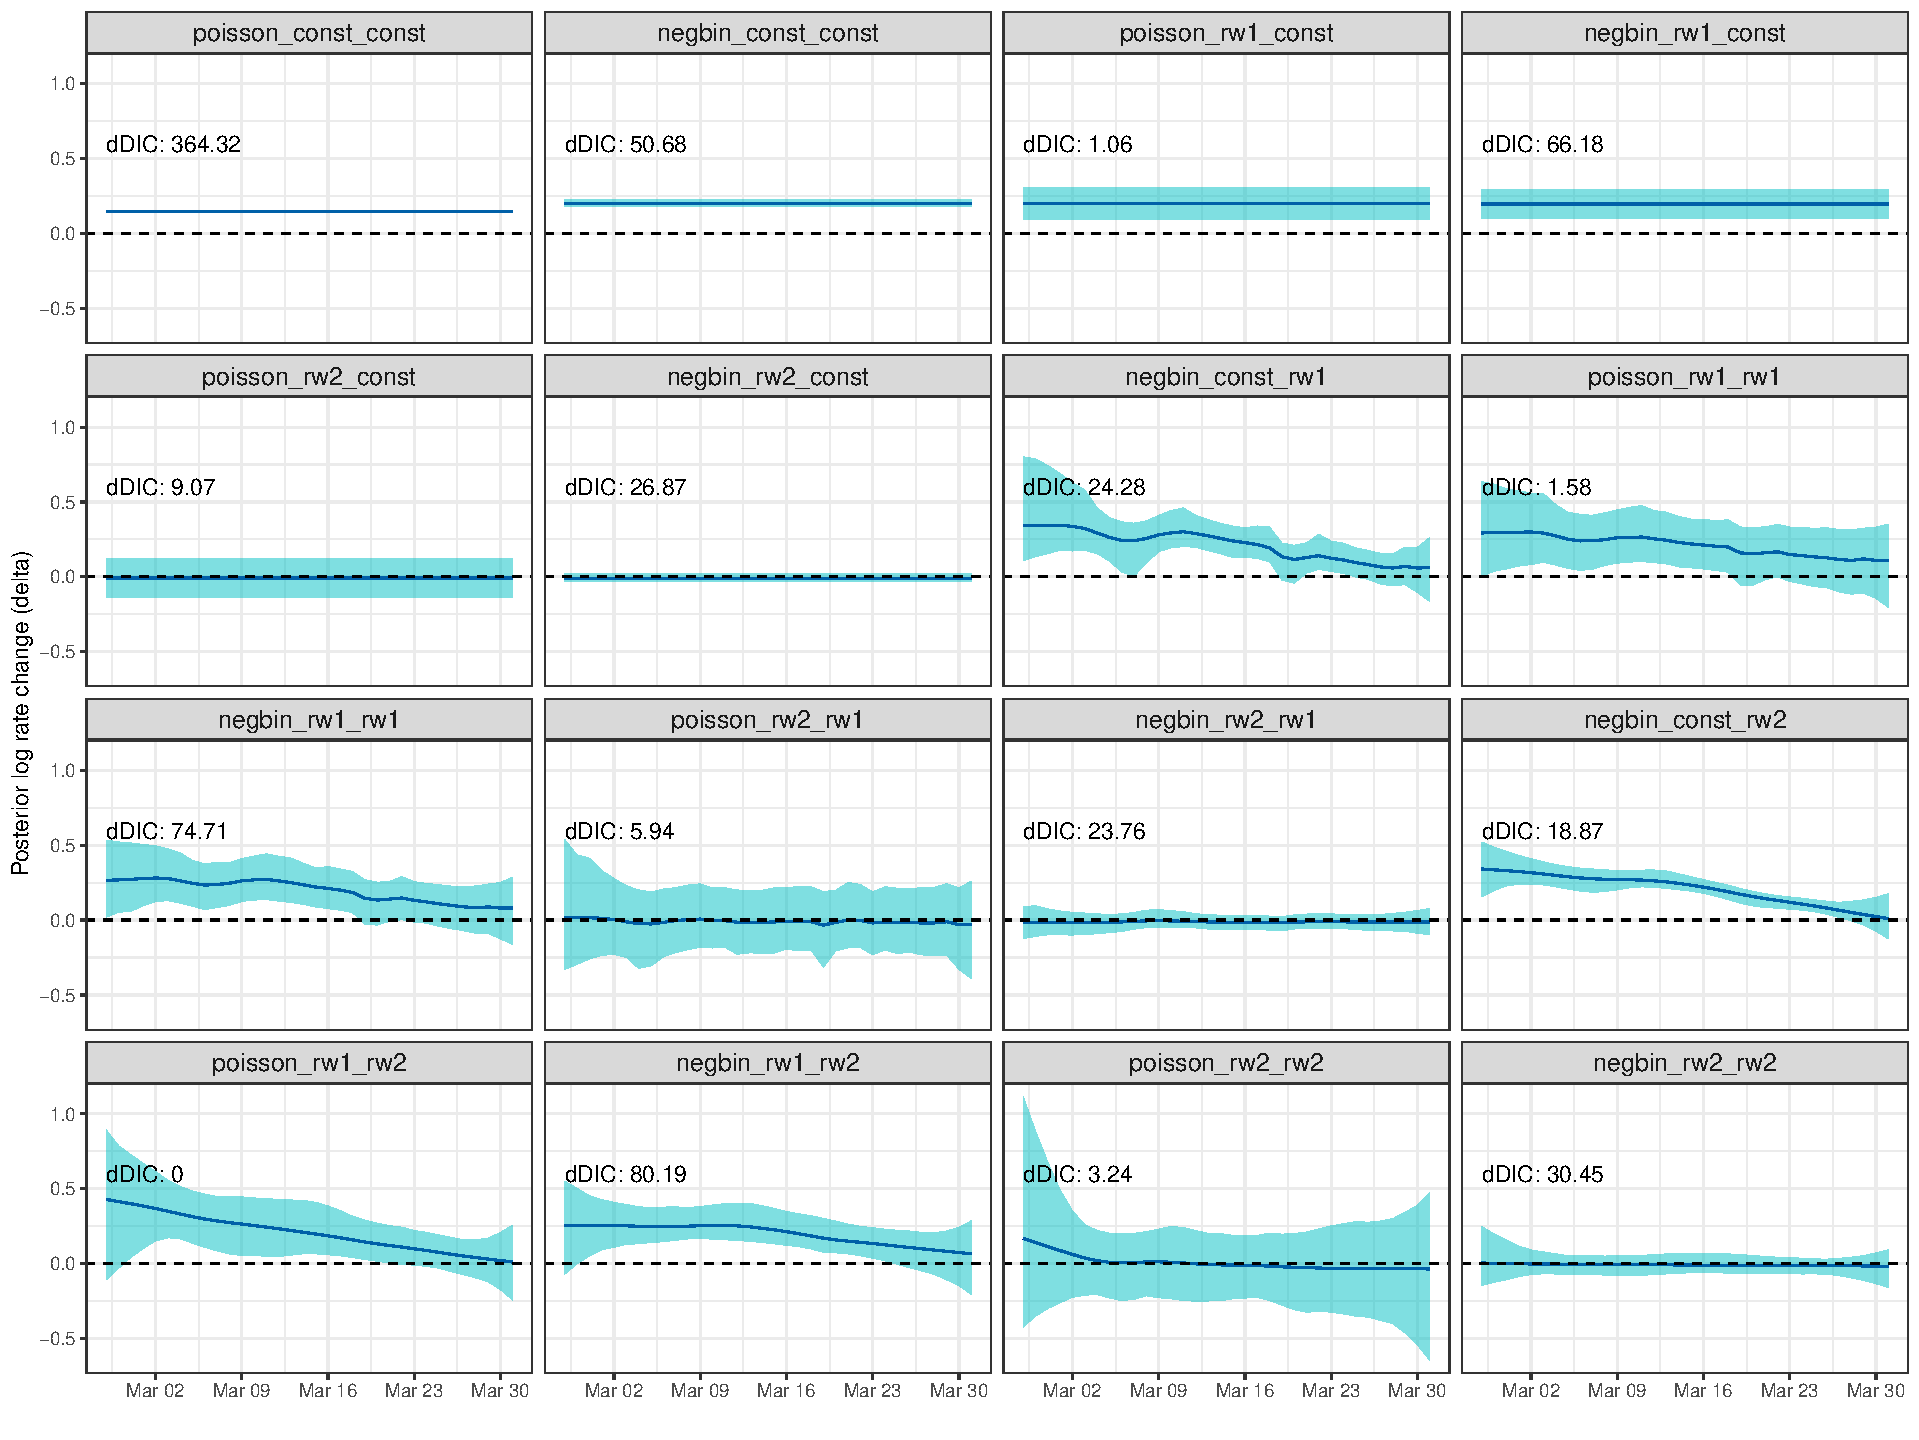
\includegraphics[width=\paperwidth]{figures/all_deltas_ireland.pdf}}
\begin{frame}[plain]
\end{frame}
}

{
\usebackgroundtemplate{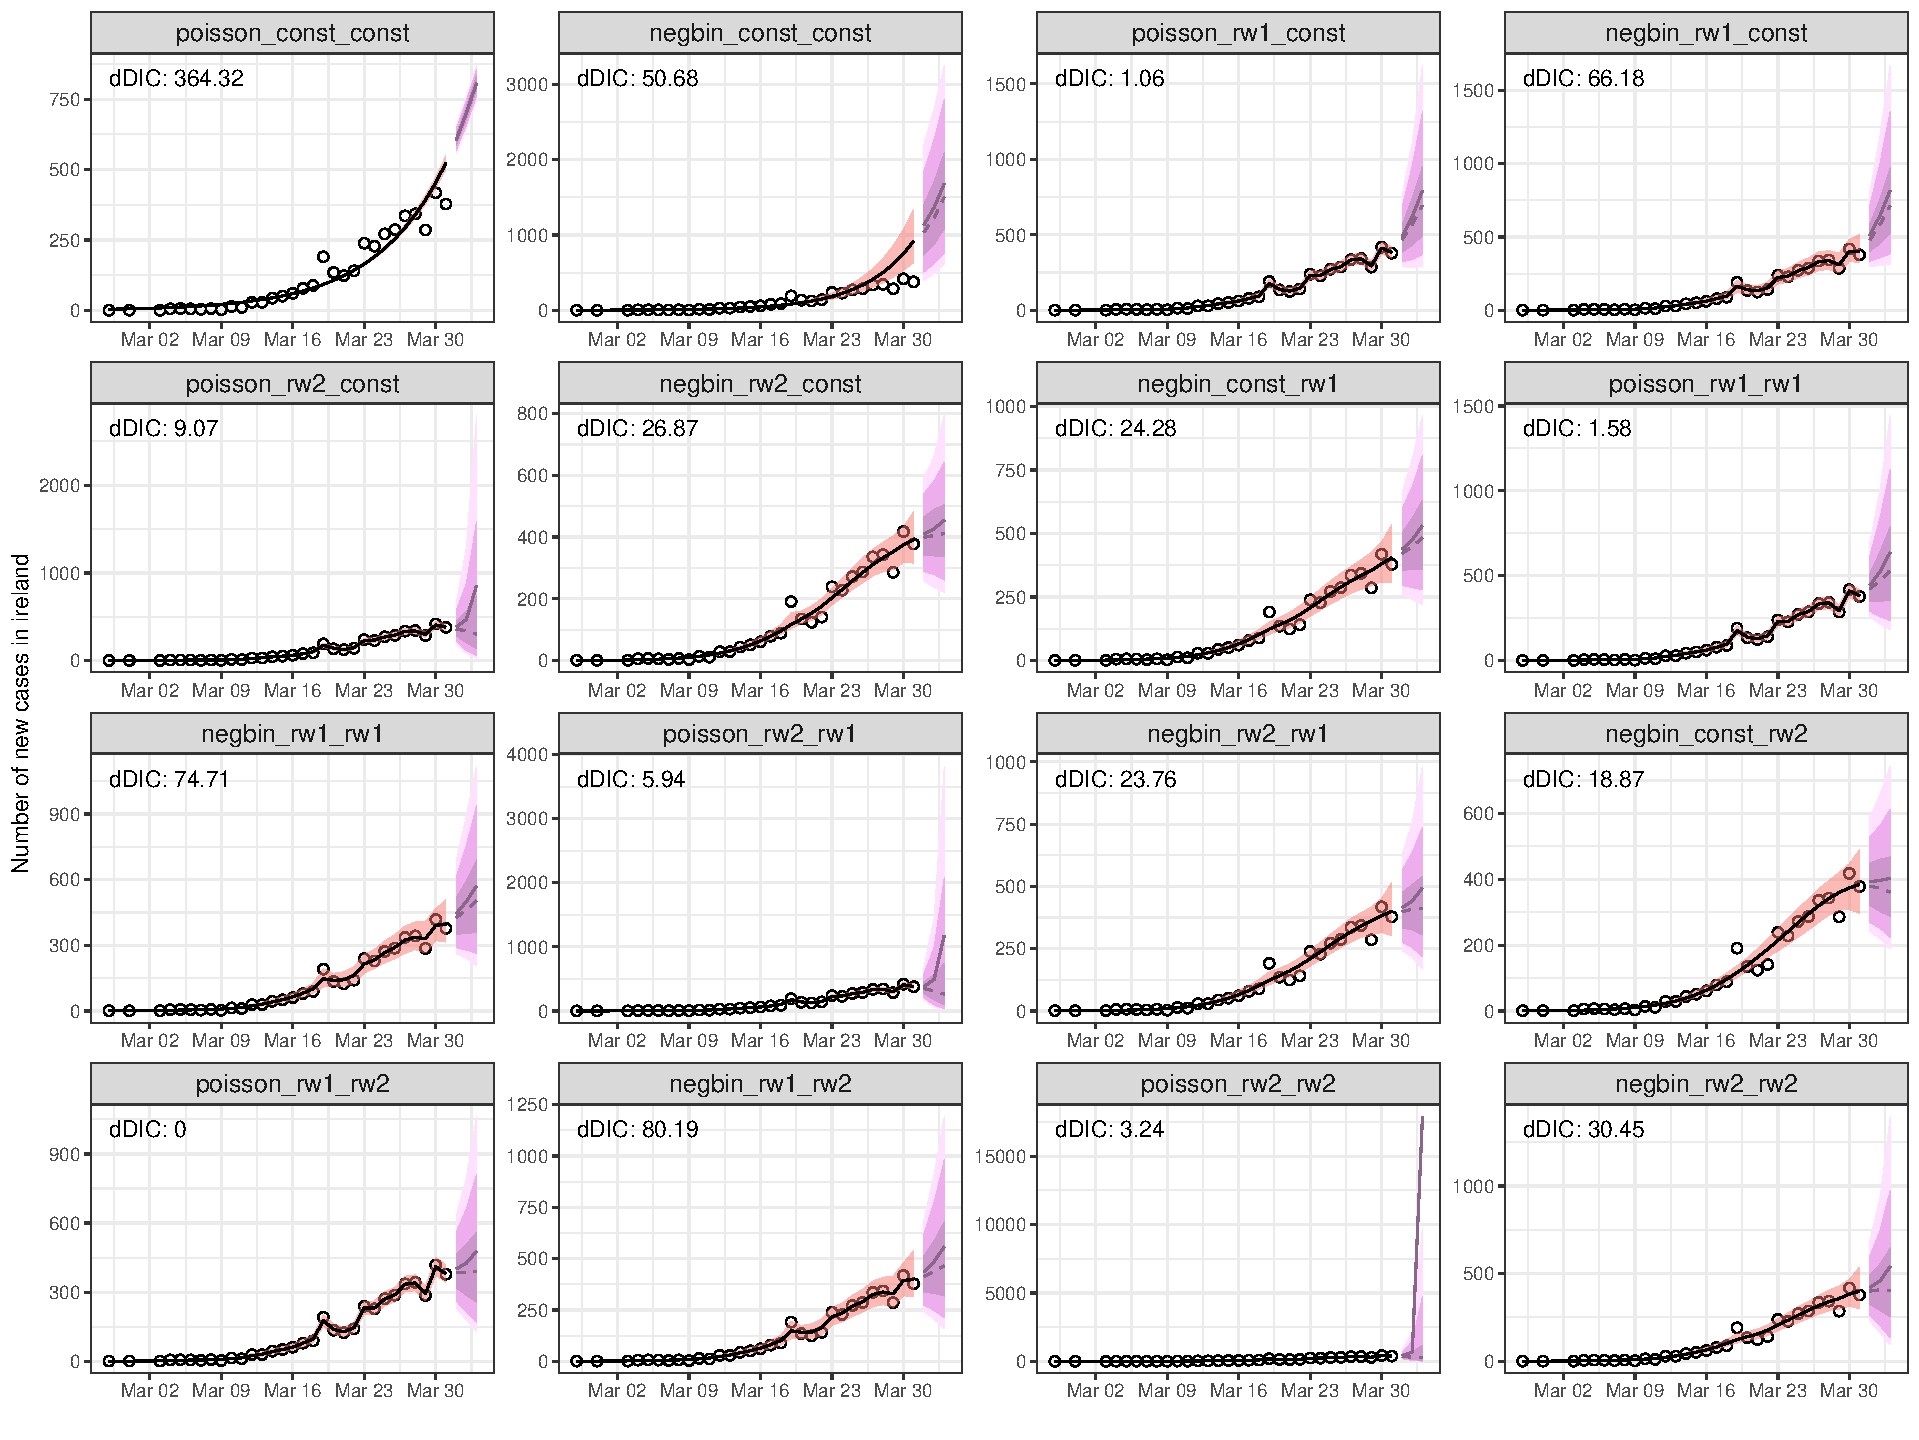
\includegraphics[width=\paperwidth]{figures/all_pred_ireland.pdf}}
\begin{frame}[plain]
\end{frame}
}

{
\usebackgroundtemplate{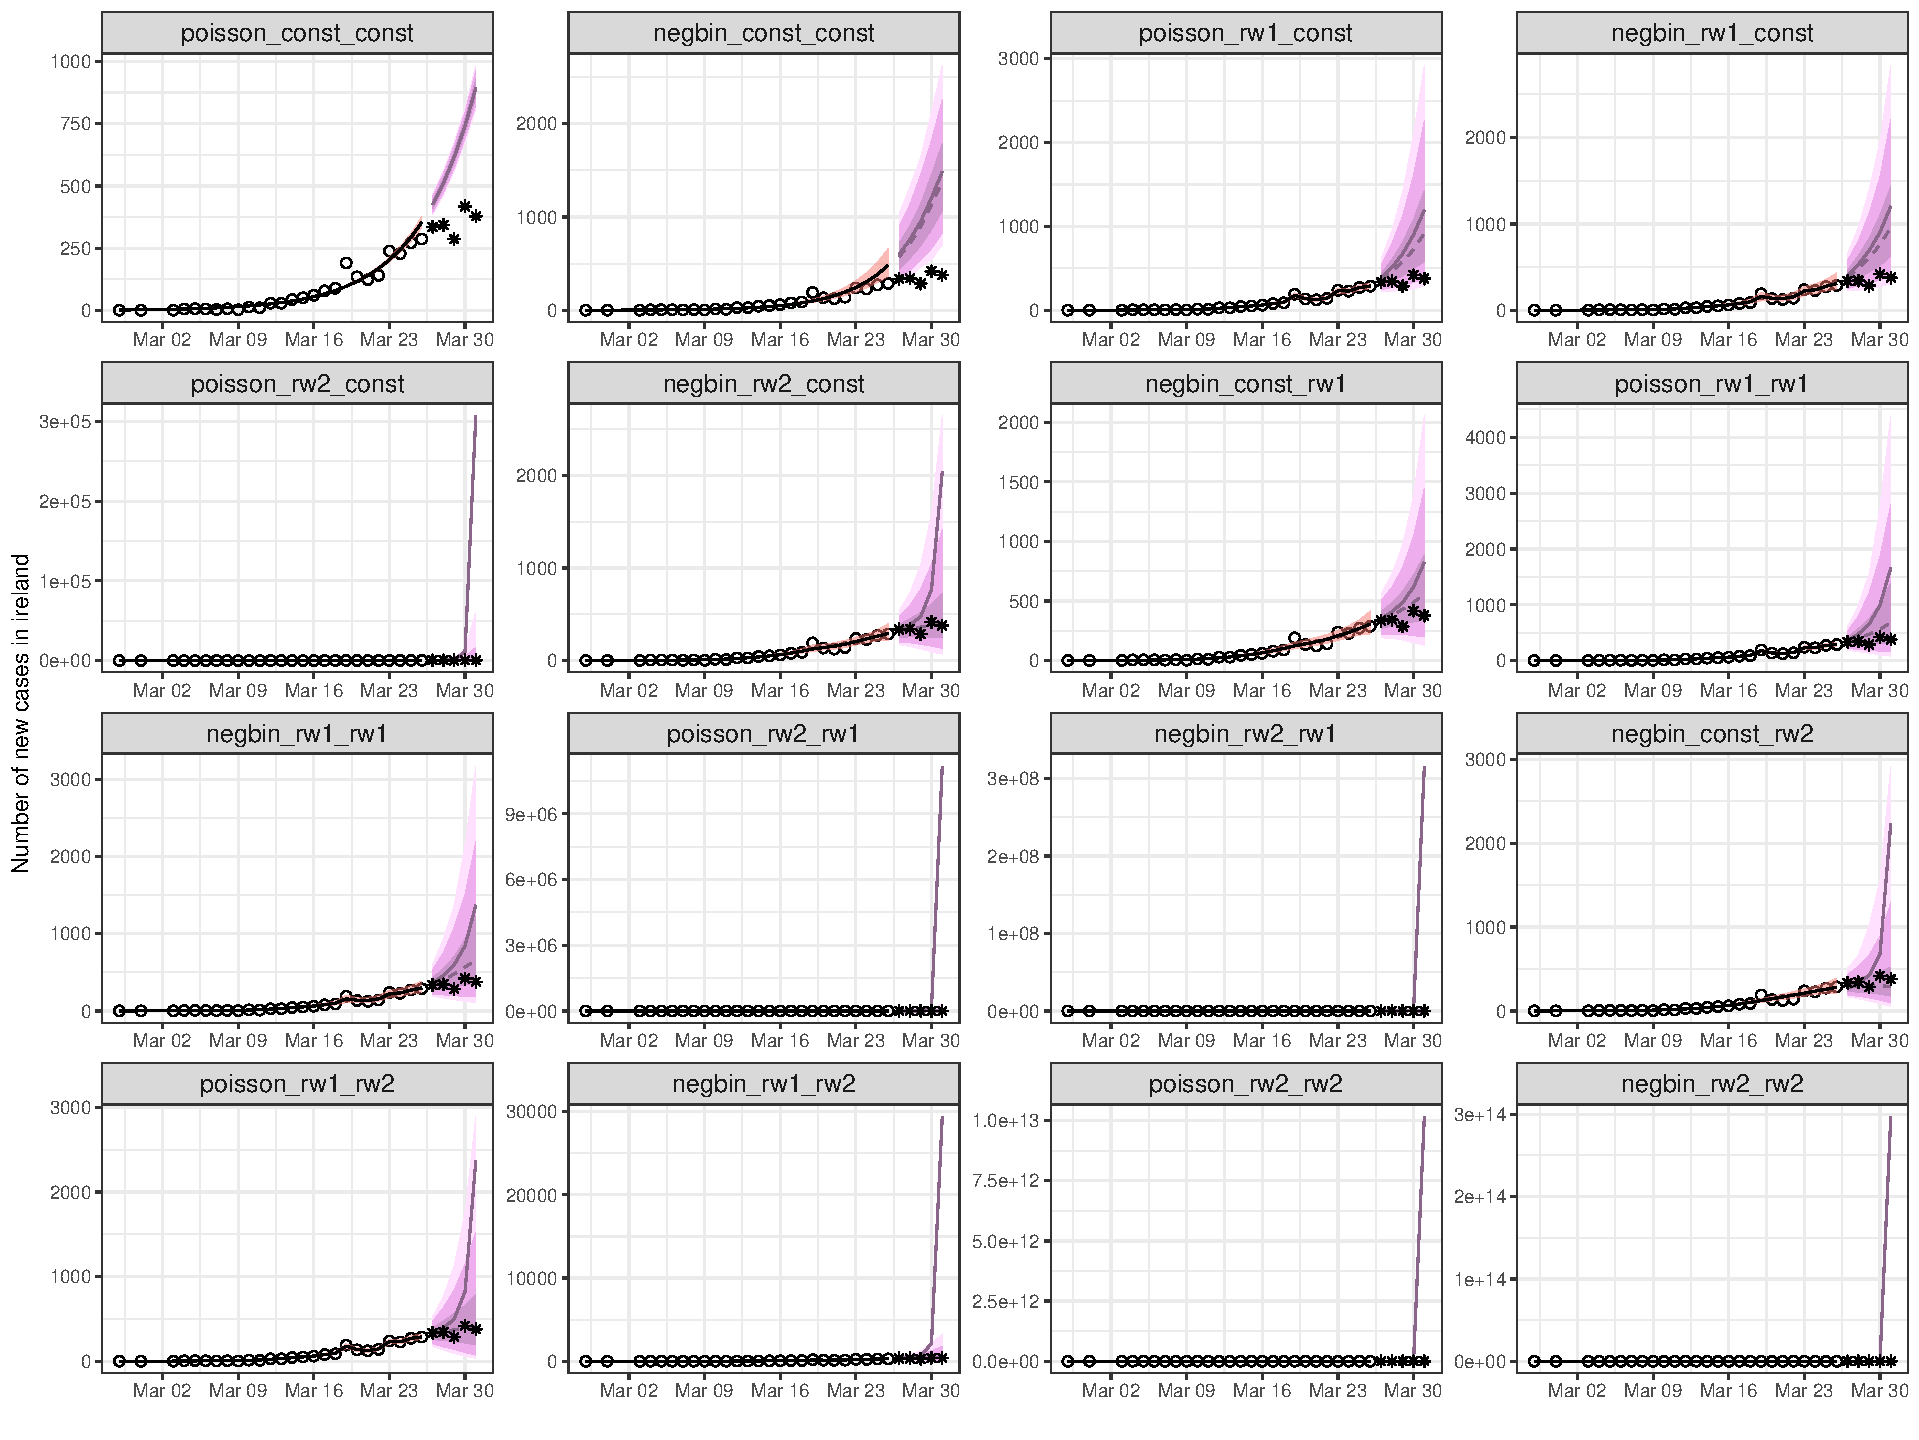
\includegraphics[width=\paperwidth]{figures/all_fits_hold_ireland.pdf}}
\begin{frame}[plain]
\end{frame}
}

\begin{frame}
\begin{figure}
 \begin{center}
  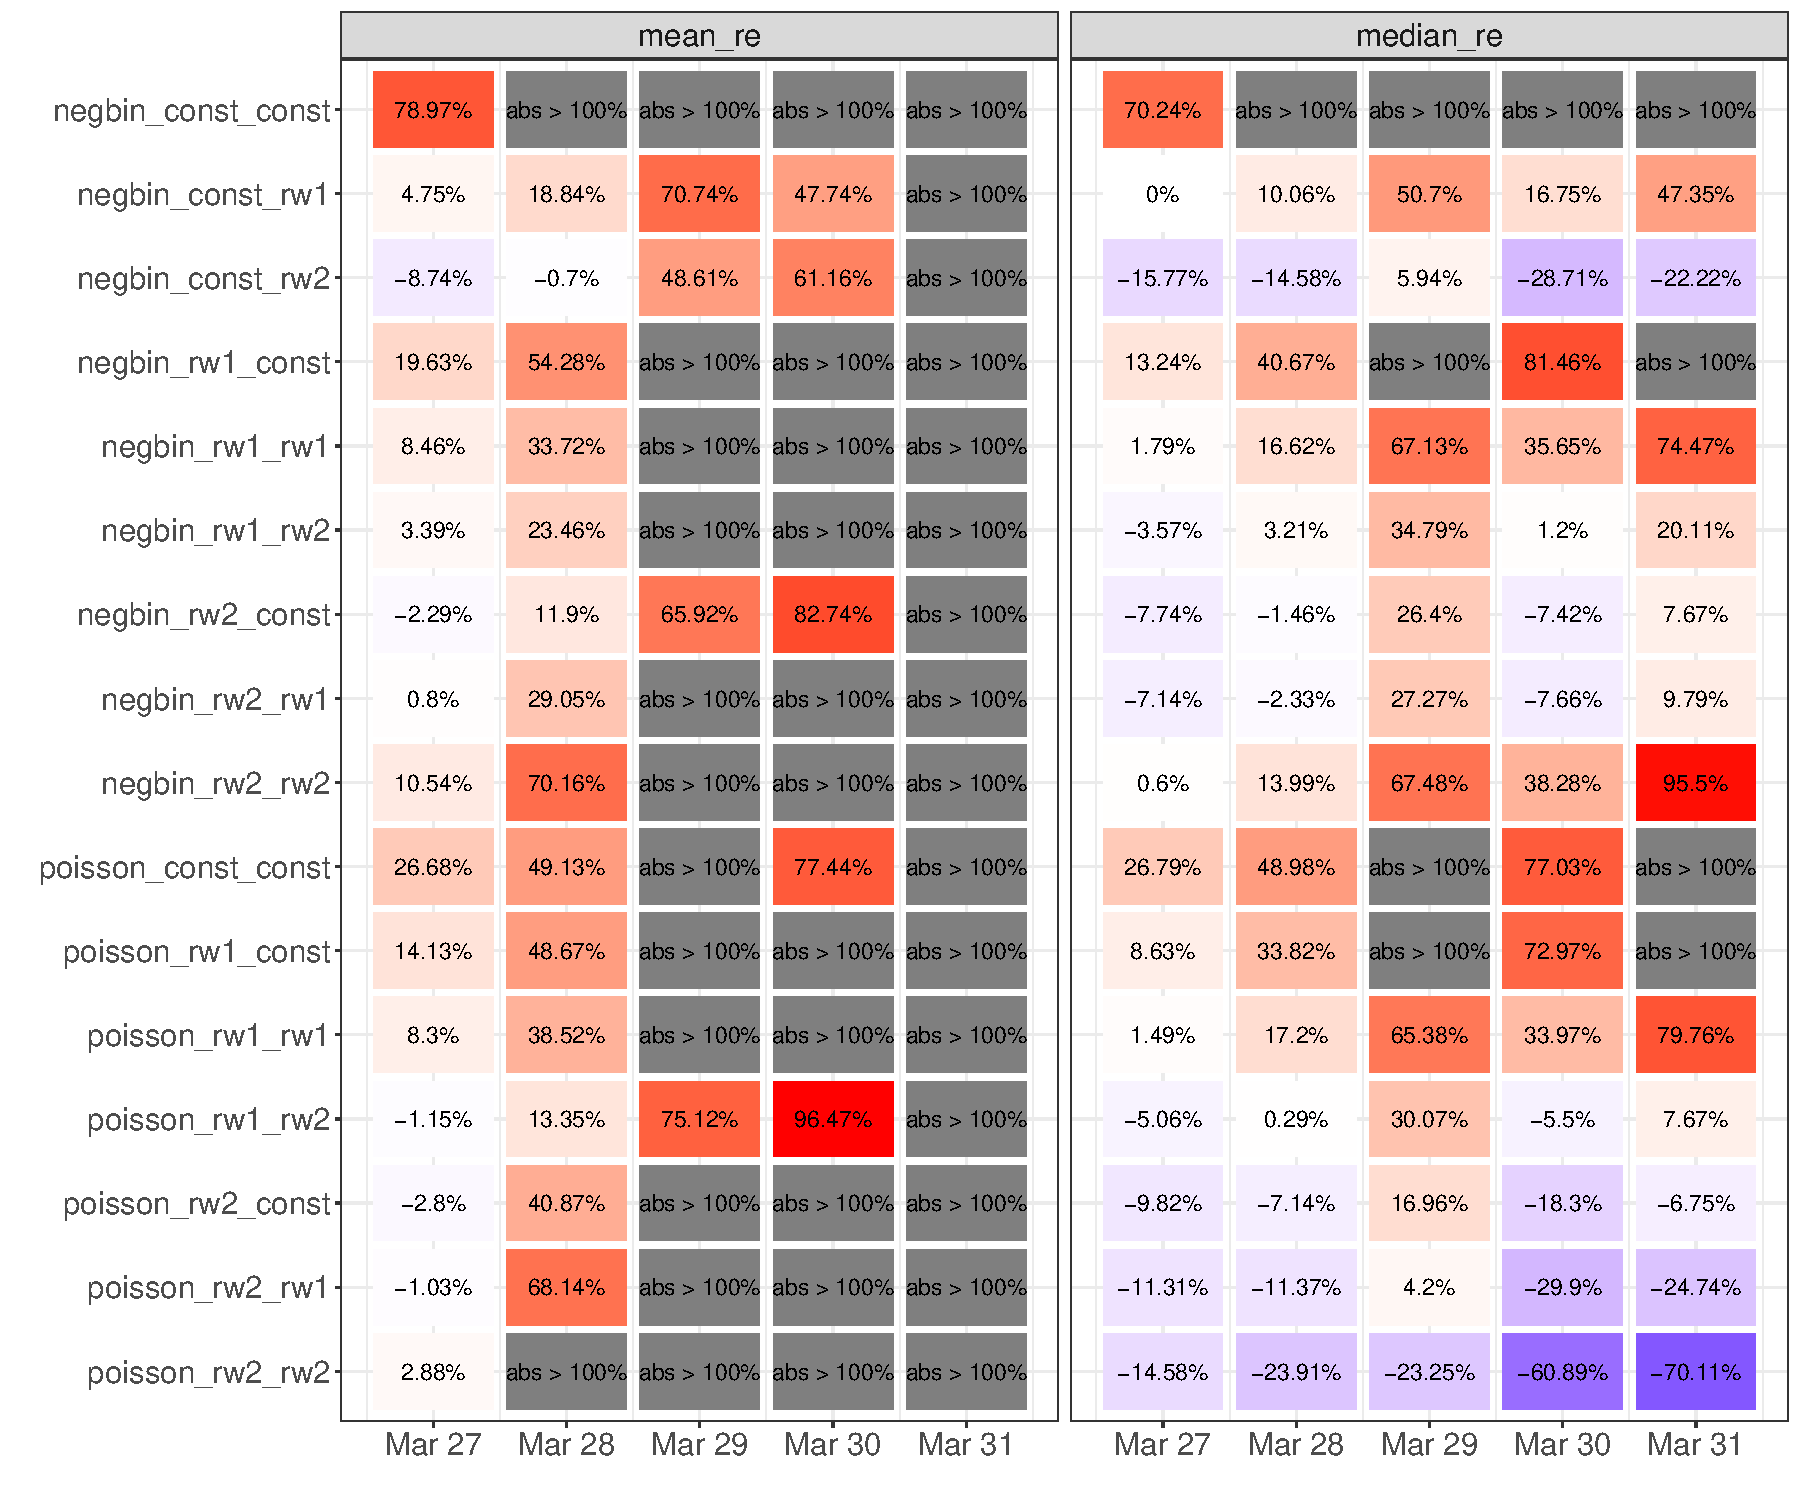
\includegraphics[height = 9cm]{figures/mdiff_hold_ireland.pdf}
 \end{center}
\end{figure}

\end{frame}

\begin{frame}
 Italy
\end{frame}

{
\usebackgroundtemplate{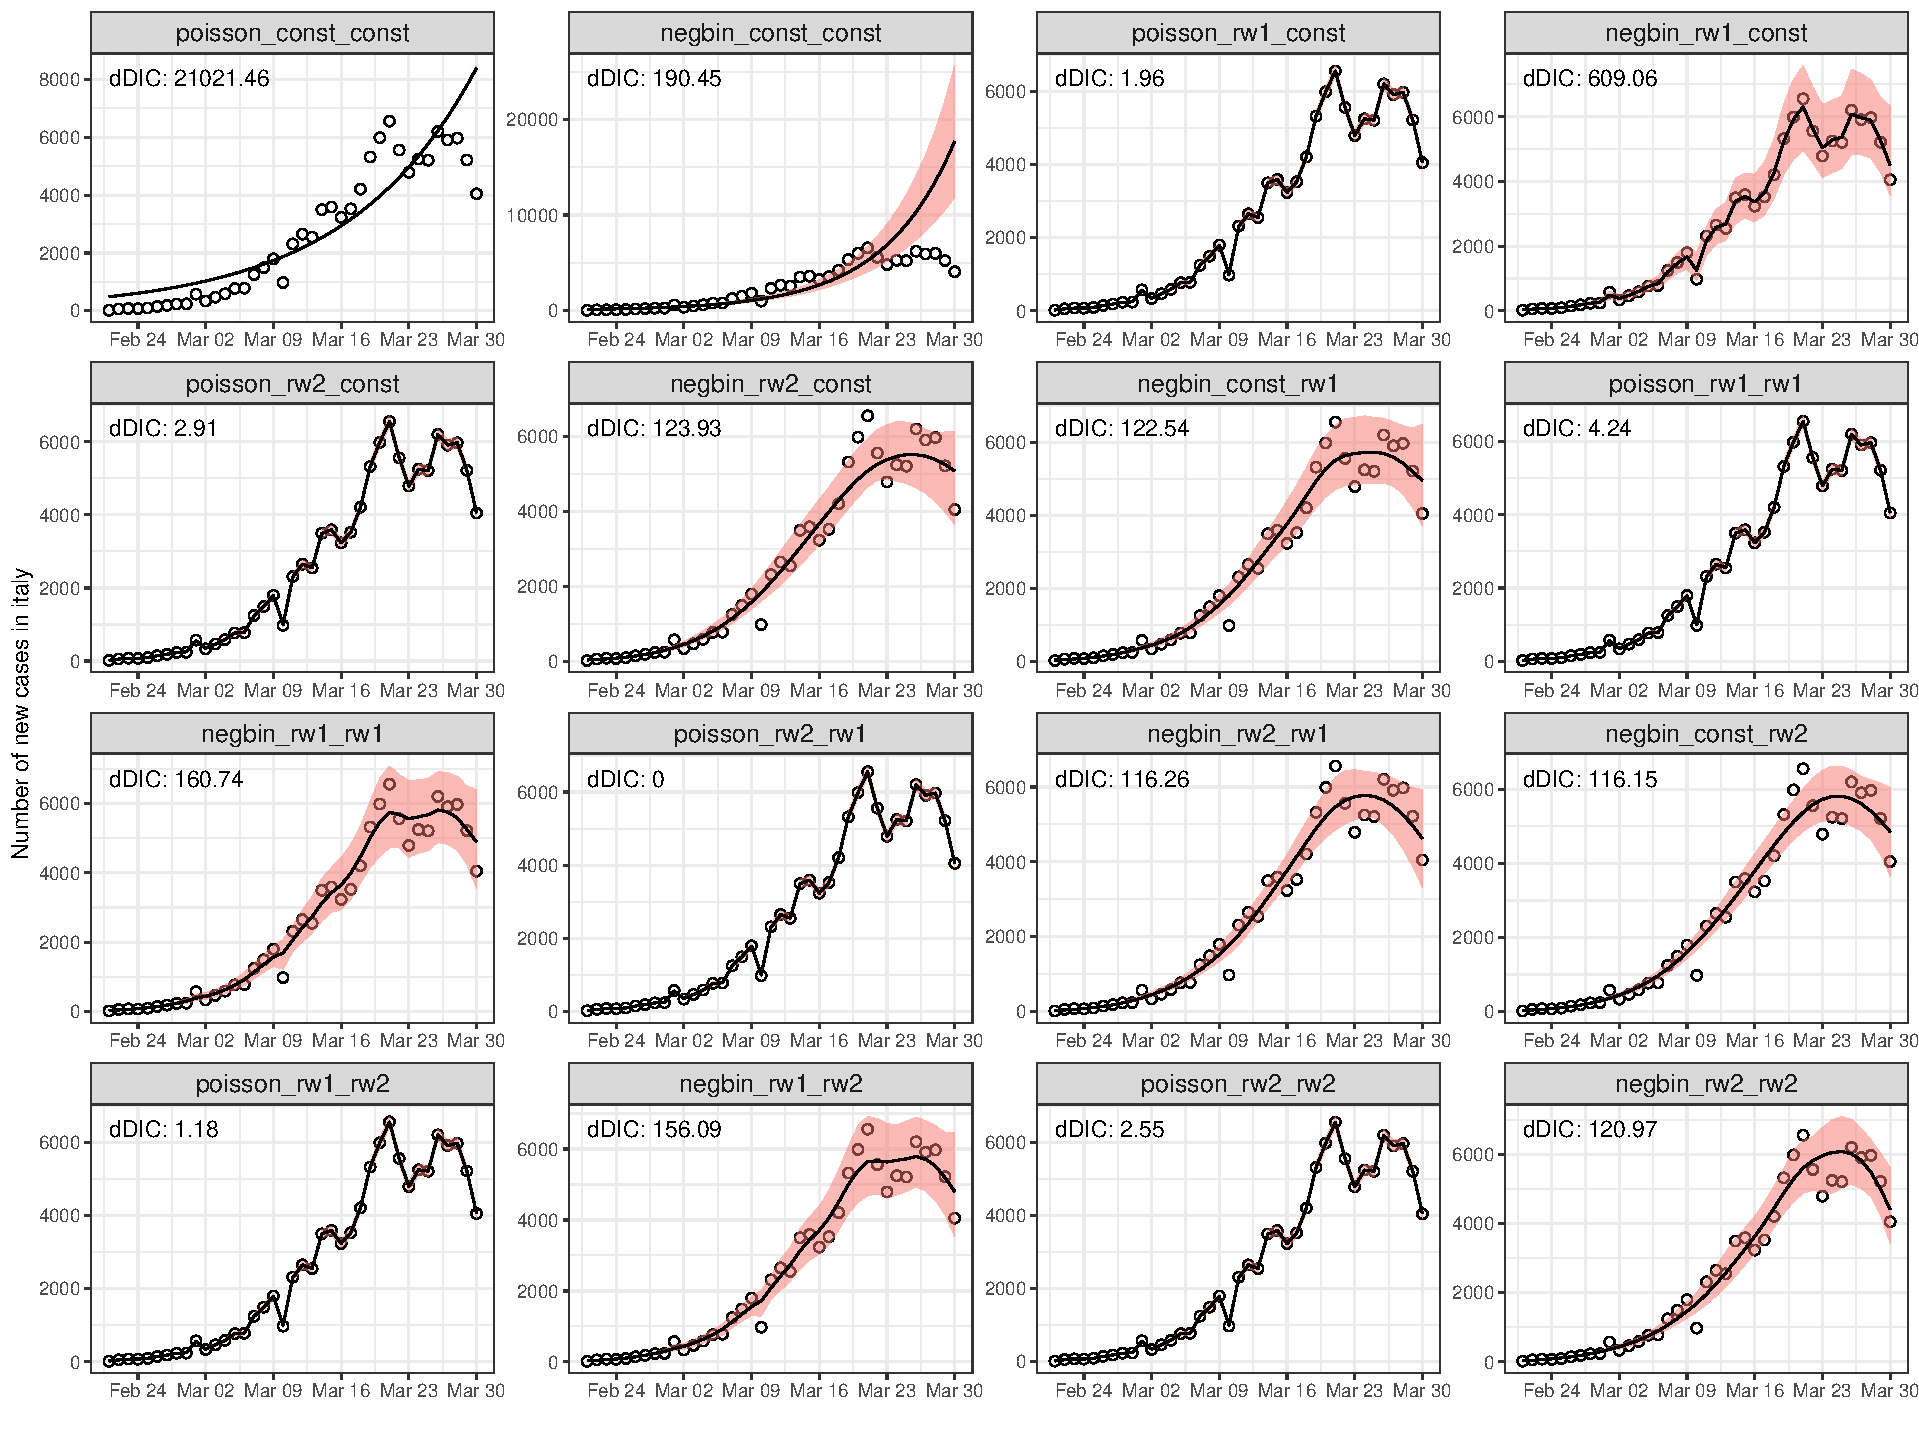
\includegraphics[width=\paperwidth]{figures/all_fits_italy.pdf}}
\begin{frame}[plain]
\end{frame}
}

{
\usebackgroundtemplate{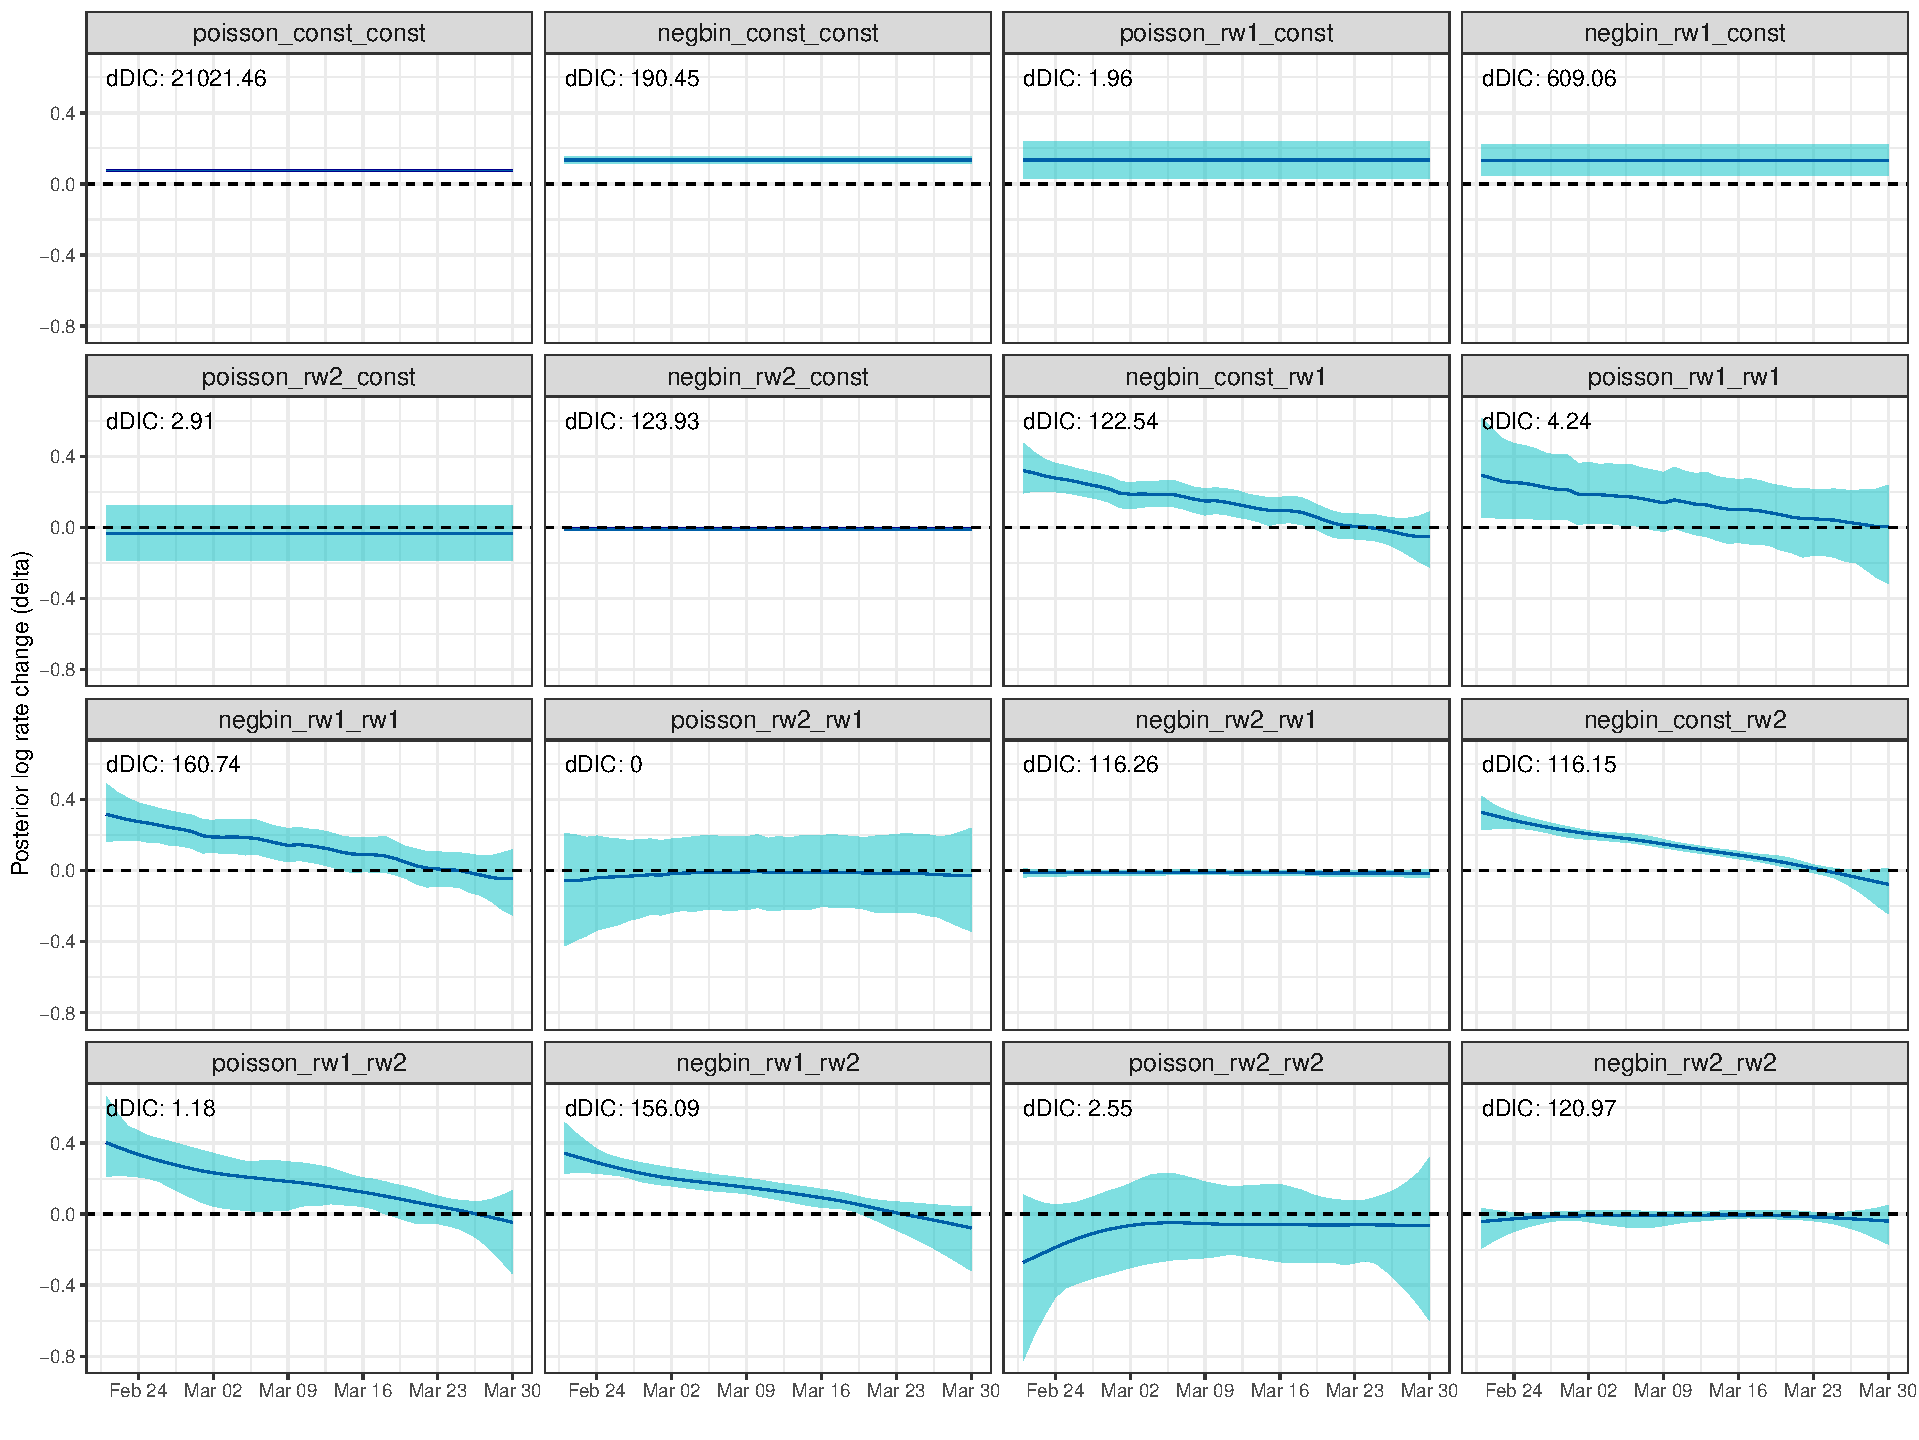
\includegraphics[width=\paperwidth]{figures/all_deltas_italy.pdf}}
\begin{frame}[plain]
\end{frame}
}

{
\usebackgroundtemplate{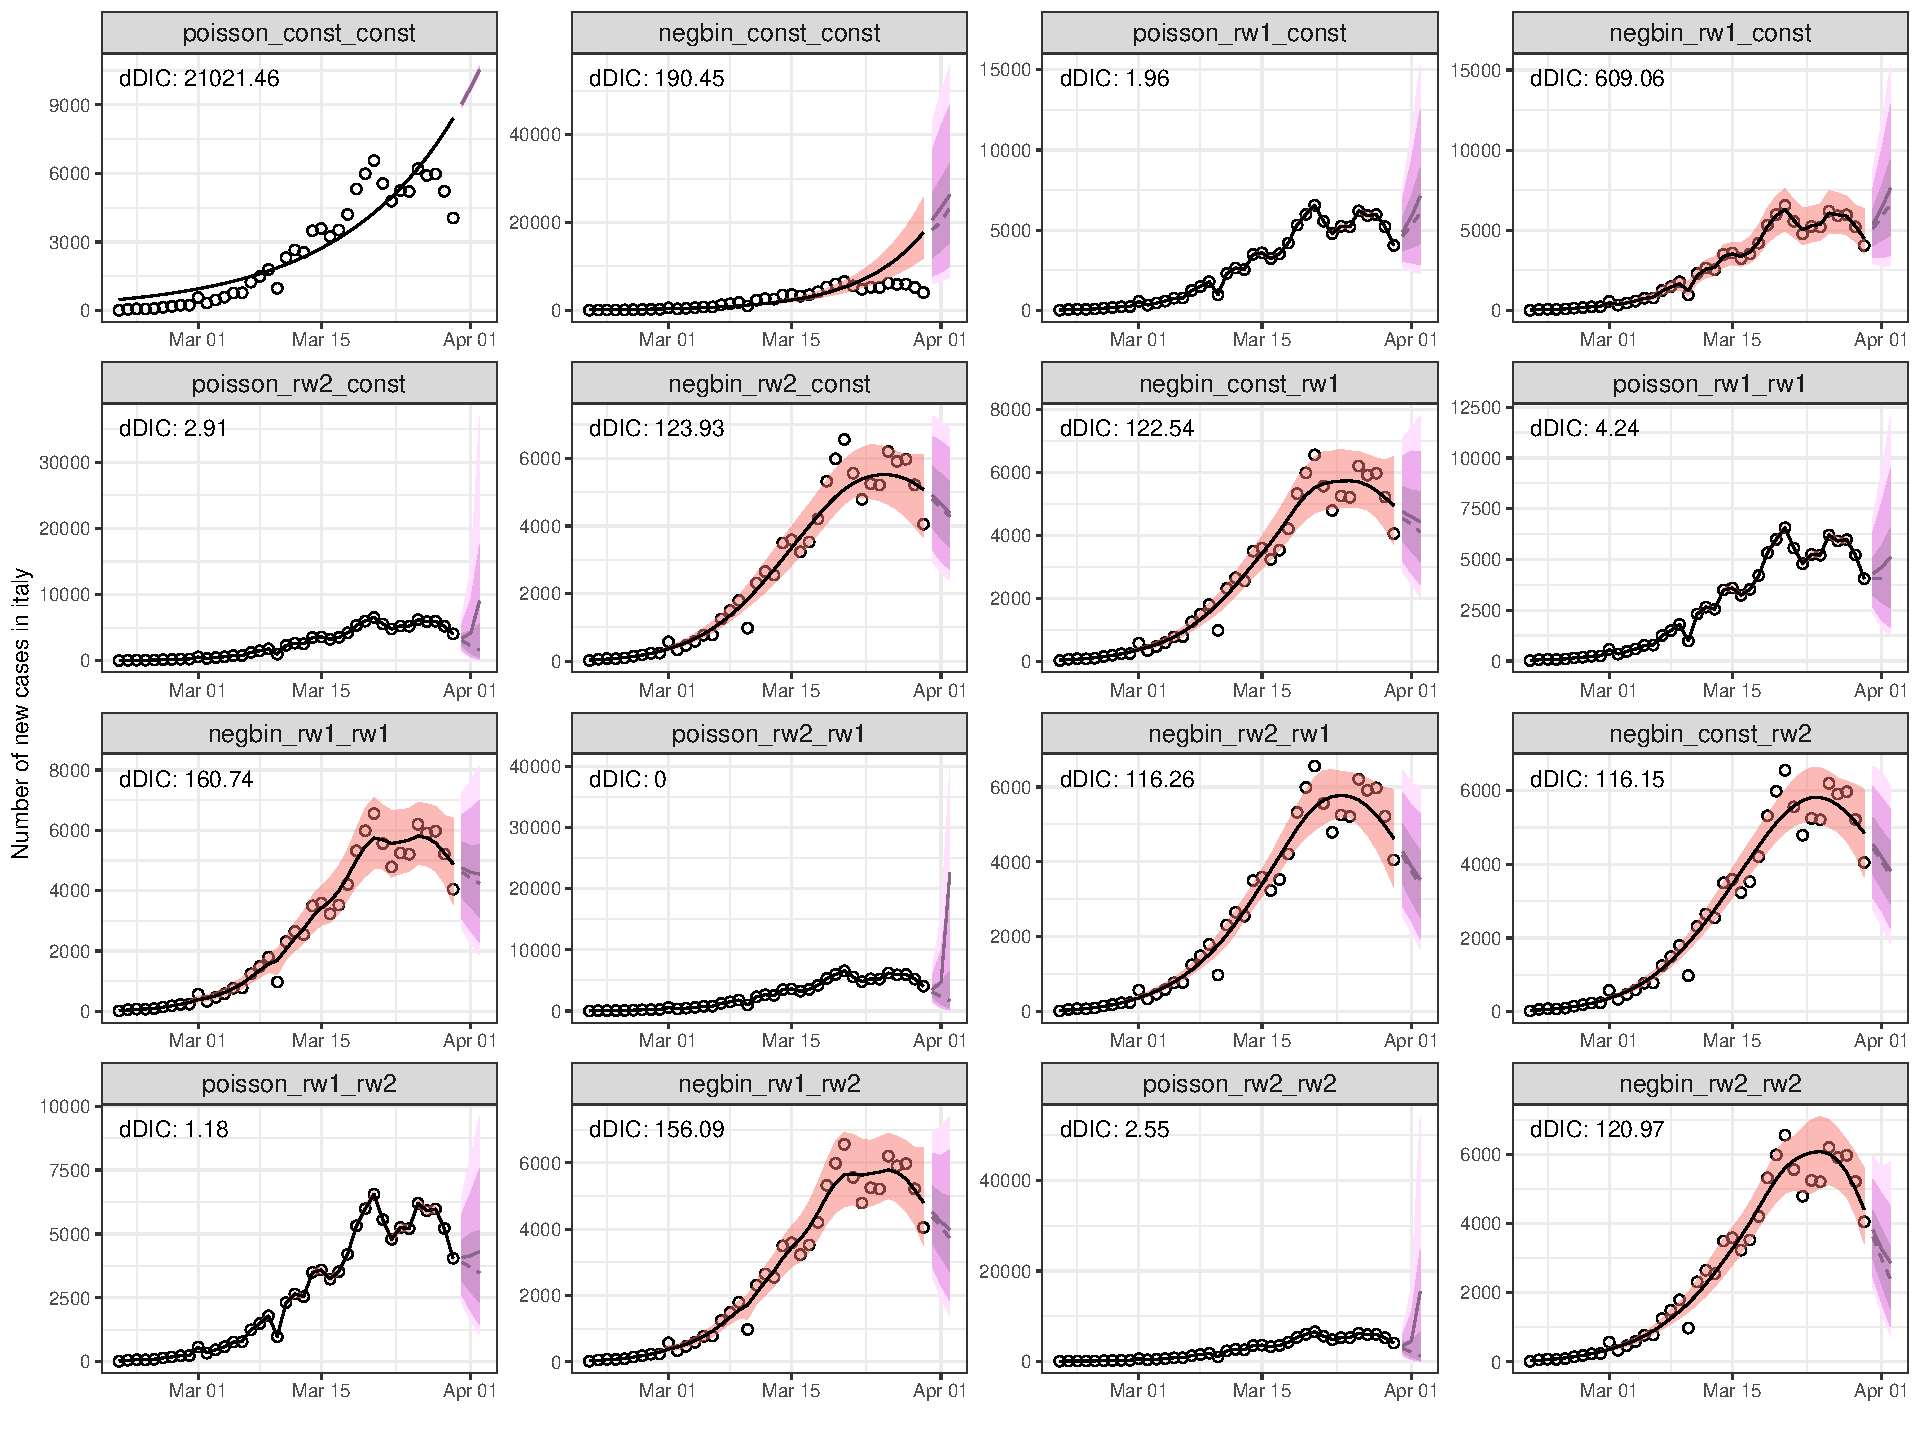
\includegraphics[width=\paperwidth]{figures/all_pred_italy.pdf}}
\begin{frame}[plain]
\end{frame}
}

{
\usebackgroundtemplate{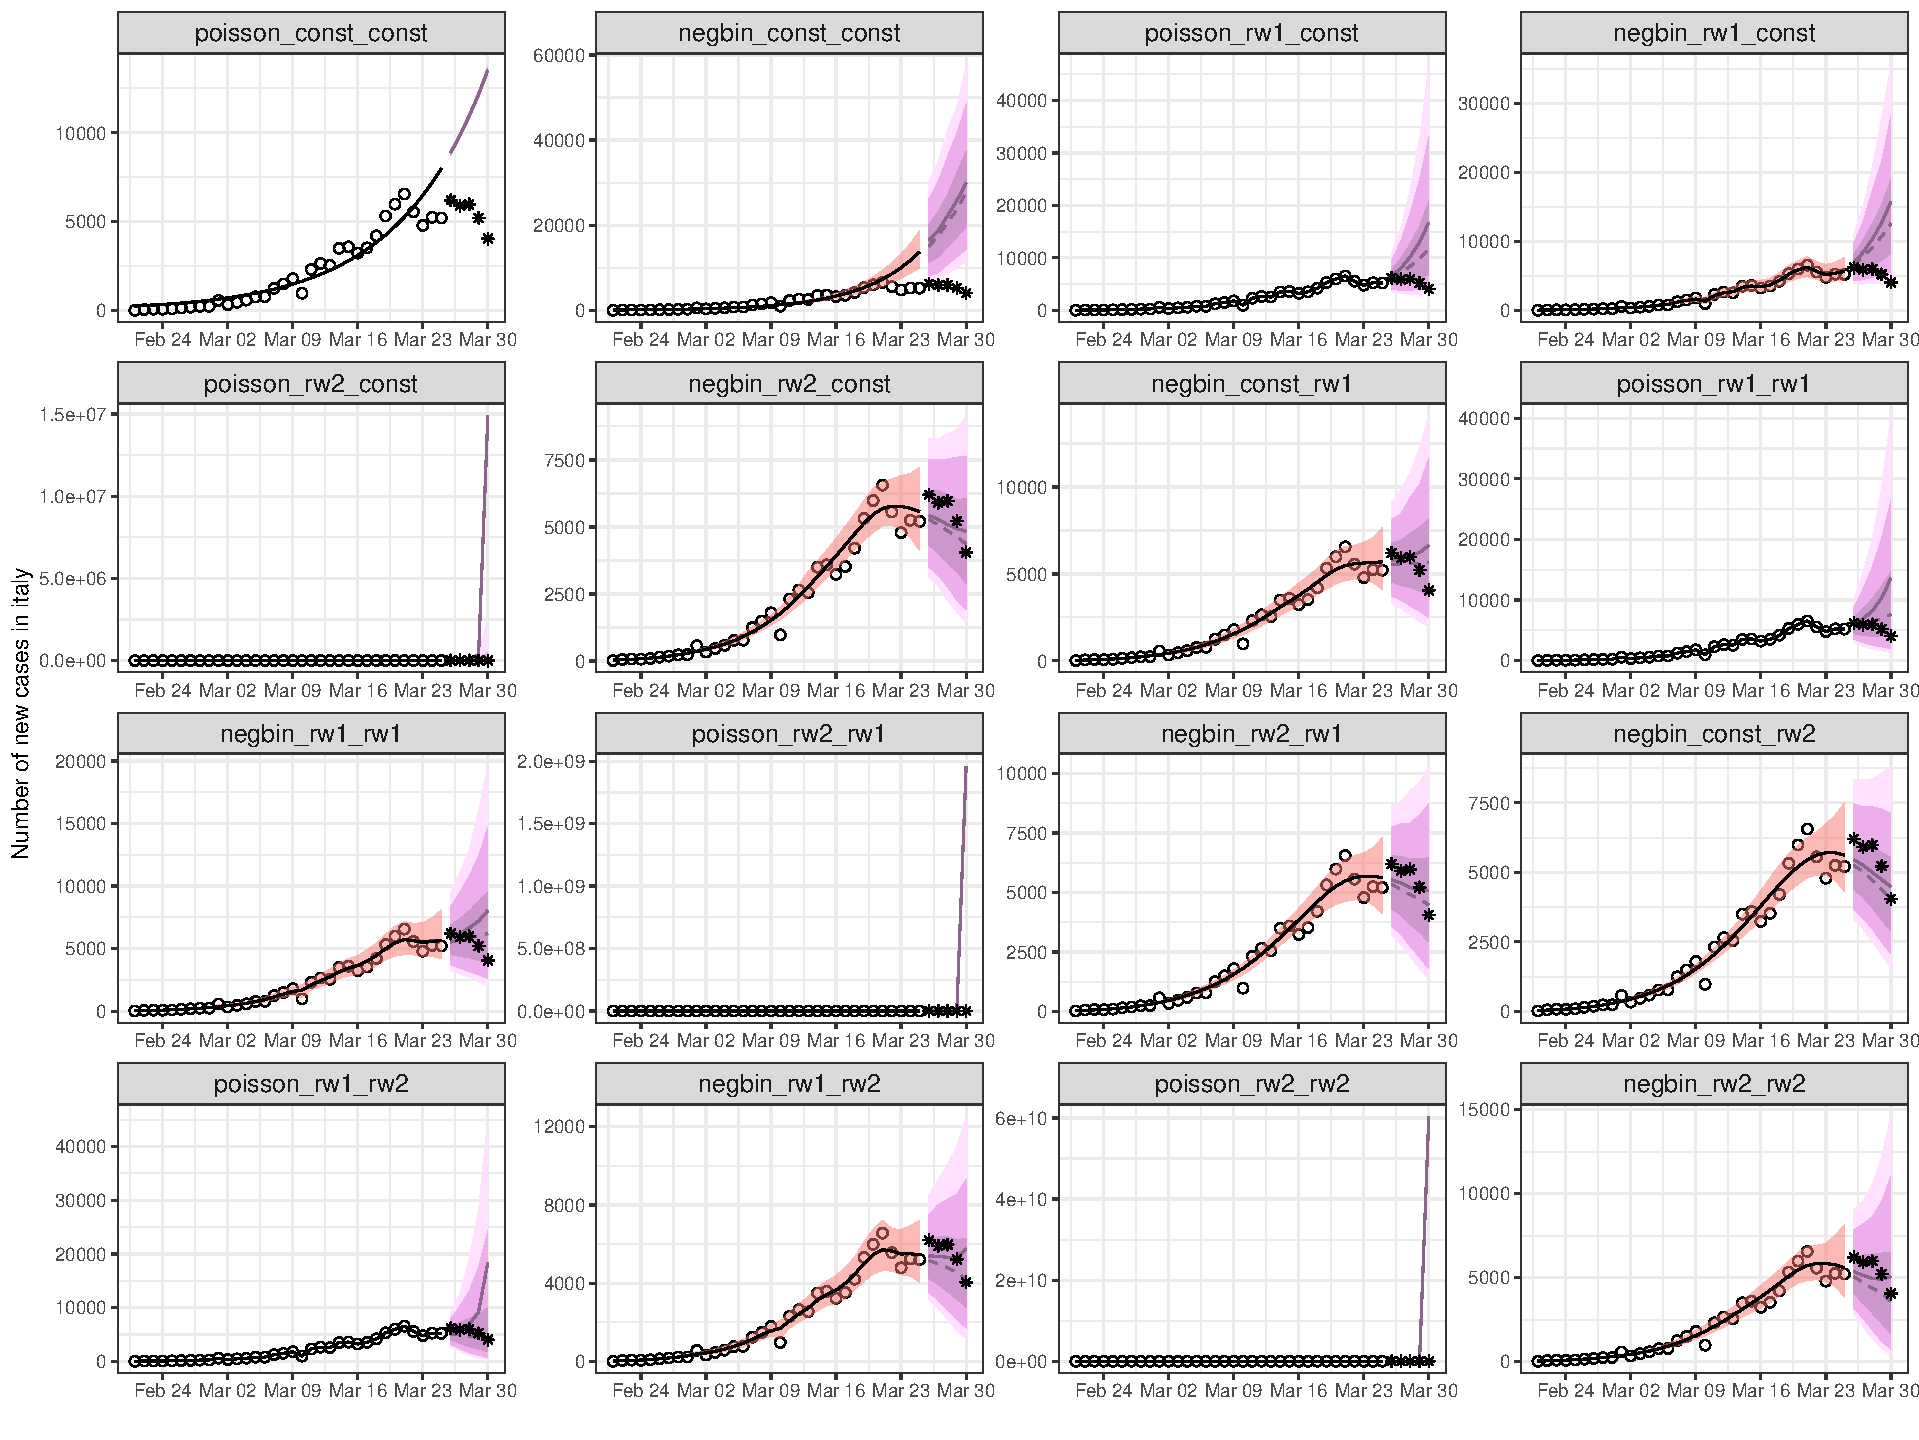
\includegraphics[width=\paperwidth]{figures/all_fits_hold_italy.pdf}}
\begin{frame}[plain]
\end{frame}
}

\begin{frame}
\begin{figure}
 \begin{center}
  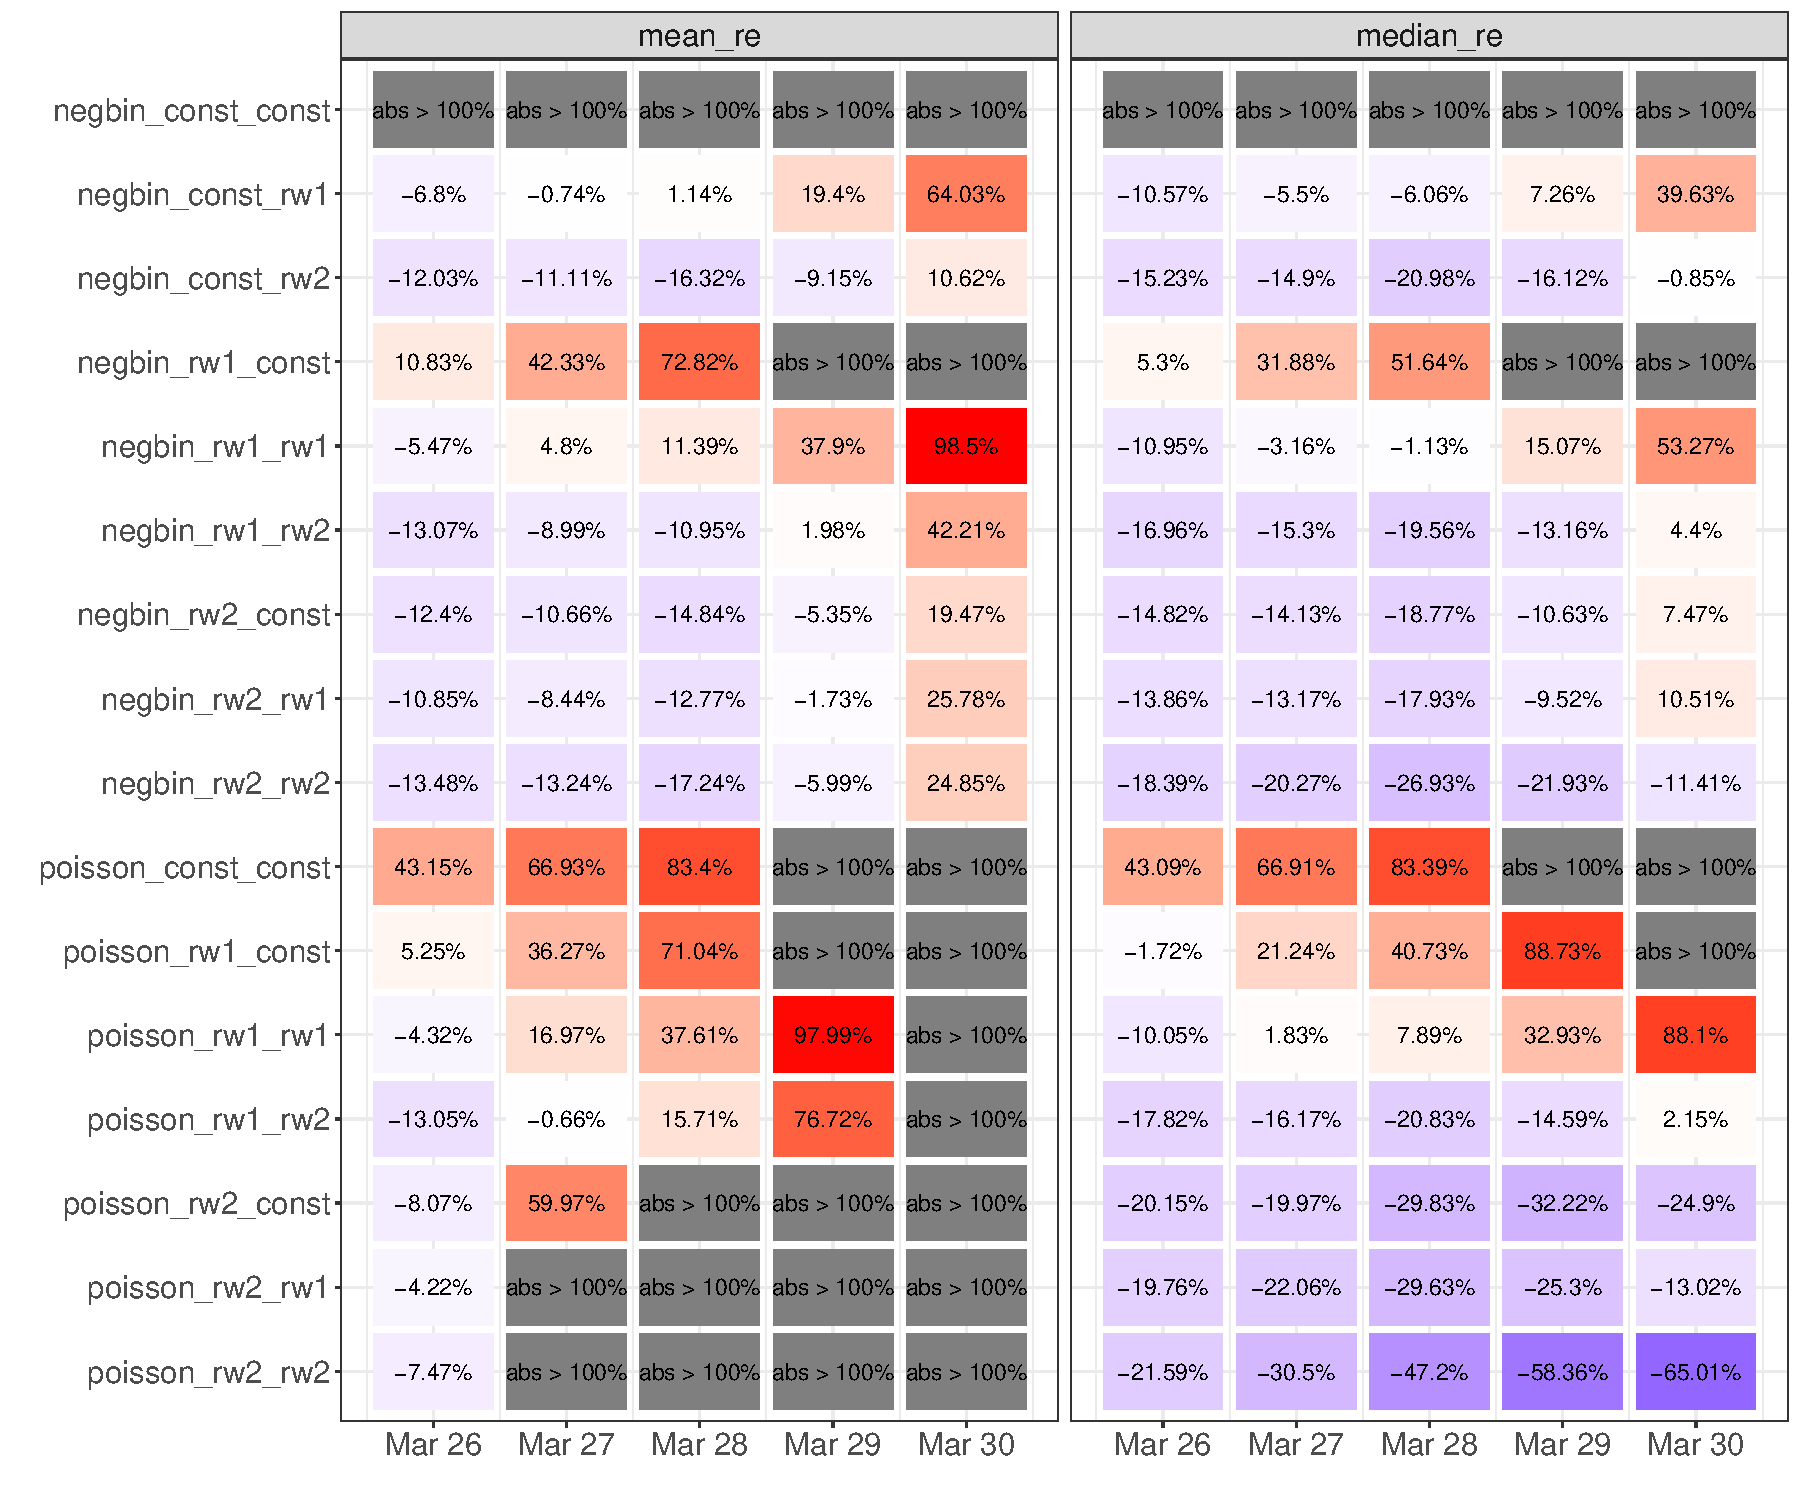
\includegraphics[height = 9cm]{figures/mdiff_hold_italy.pdf}
 \end{center}
\end{figure}
\end{frame}

\end{document}


\begin{frame}
 \frametitle{}
\end{frame}


